% ОБЯЗАТЕЛЬНО ИМЕННО ТАКОЙ documentclass!
% (Основной кегль = 14pt, поэтому необходим extsizes)
% Формат, разумеется, А4
% article потому что стандарт не подразумевает разделов
% Глава = section, Параграф = subsection
% (понятия "глава" и "параграф" из документа, описывающего диплом)
\documentclass[a4paper,article,14pt]{extarticle}

% Подключаем главный пакет со всем необходимым
\usepackage{styles}

% Пакеты по желанию (самые распространенные)
% Хитрые мат. символы
\usepackage{euscript}
% Таблицы
\usepackage{longtable}
\usepackage{makecell}
% Картинки (можно встявлять даже pdf)
\usepackage[pdftex]{graphicx}

\usepackage{amsthm,amssymb, amsmath}
\usepackage{textcomp}
\usepackage{amsmath}
\usepackage{csquotes}


\begin{document}

% Титульник
    % Временное удаление foot на titlepage
\newgeometry{left=30mm, top=20mm, right=15mm, bottom=20mm, nohead, nofoot}
\begin{titlepage}
    \begin{center}
        \textbf{Министерство науки и высшего образования Российской Федерации}
        \linebreak
        \textnormal{ФЕДЕРАЛЬНОЕ ГОСУДАРСТВЕННОЕ АВТОНОМНОЕ ОБРАЗОВАТЕЛЬНОЕ УЧРЕЖДЕНИЕ ВЫСШЕГО ОБРАЗОВАНИЯ}
        \textbf{НАЦИОНАЛЬНЫЙ ИССЛЕДОВАТЕЛЬСКИЙ УНИВЕРСИТЕТ ИТМО}
        \textquotedblright
        \linebreak
        \vspace{35mm}

        \textnormal{ОТЧЕТ О ПРАКТИЧЕСКОЙ РАБОТЕ}
        \linebreak
        \textbf{по дисциплине \enquote{Проектная документация}}
        \linebreak
        \textbf{по теме: \enquote{Сопровождение и техническая поддержка}}
        \linebreak
    \end{center}

        \vspace{35mm}
    \normalsize{
        \begin{tabular}{cccc}
            Руководитель & \underline{\hspace{3cm}} & Повышев Владислав Вячеславович \\\\
        \end{tabular}
    }\\
    \begin{center}
        \textbf{СПИСОК ИСПОЛНИТЕЛЕЙ}
    \end{center}

    \normalsize{
        \begin{tabular}{cccc}
            Выполнил & \underline{\hspace{3cm}} & Ярощук Владислав Викторович
        \end{tabular}
    }
% Название

    \begin{center}
%        \vspace{20mm}
        \vfill
        {Санкт-Петербург}
        \par{\the\year{} г.}
    \end{center}
\end{titlepage}
% Возвращаем настройки geometry обратно (то, что объявлено в преамбуле)
\restoregeometry
% Добавляем 1 к счетчику страниц ПОСЛЕ titlepage, чтобы исключить
% влияние titlepage environment
\addtocounter{page}{1}


% Реферат
    %! Author = vladislav.yaroshchuk
%! Date = 10/10/2021

\pagebreak
\begin{center}
    \specialsection{Реферат}
\end{center}

% Содержание
    \pagebreak
    \tableofcontents

% Введение
    %! Author = vladislav.yaroshchuk
%! Date = 10/10/2021

\pagebreak
\specialsection{Введение}

Введение Введение Введение
Введение Введение Введение
Введение Введение Введение


% Основная часть
    %! Author = vladislav.yaroshchuk
%! Date = 10/10/2021

\pagebreak


\section{Формирование перечня стандартов.}

Для выполнения практикума был сформирован перечень стандартов документирования этапа \enquote{Сопровождение и техническая поддержка}:

\begin{itemize}
    \item ГОСТ Р ИСО/МЭК 14764--2002 Информационная технология.
    Сопровождение программных средств.

    \item ГОСТ Р ИСО/МЭК 9126--93 Информационная технология.
    Оценка программной продукции.
    Характеристика качества и руководства по их применению.

    \item ГОСТ Р ИСО/МЭК 20000-1-2013 Информационная технология.
    Управление услугами.
    Часть 1.
    Требования к системе управления услугами.

    \item ГОСТ Р ИСО/МЭК 12207--2010 Информационная технология.
    Процессы жизненного цикла программных средств.

    \item ГОСТ Р ИСО/МЭК 9126--93 Информационная технология (ИТ).
    Оценка программной продукции.
    Характеристики качества и руководства по их применению

    \item ISO 9000:2015.
    Quality management systems -- Fundamentals and vocabulary.

    \item ISO/IEC 14764:2006.
    Software Engineering -- Software Life Cycle Processes -- Maintenance.

    \item ISO/IEC 25010:2011.
    Systems and software engineering --
    Systems and software Quality Requirements and Evaluation (SQuaRE) --
    System and software quality models

    \item SWEBOK v3.0.
    Chapter 5: Software Maintenance.
\end{itemize}


    %! Author = vladislav.yaroshchuk
%! Date = 10/10/2021

\pagebreak


\section{Выделение ключевых понятий этапа жизненного цикла ПО из стандартов.}

Каждый из стандартов описывает свою область применения в рамках терминов и понятий.
После анализа выбранных стандартов были выделены следующие основные и дополнительные понятия.


Основные понятия:
\begin{enumerate}
    \item Сопровождение (maintenance)
    \begin{enumerate}
        \item модификации программного продукта в части его кода и документации
        для решения возникающих проблем при эксплуатации или реализации потребностей в
        улучшениях тех или иных характеристик.
        (ГОСТ Р ИСО/МЭК 12207-2010)
        \item modification of existing software while preserving its integrity.
        (SWEBOK v3)
    \end{enumerate}

    \item Сопровождаемость (Maintainability)
    \begin{enumerate}
        \item Набор атрибутов, относящихся к объему работ, требуемых для проведения конкретных изменений (модификаций).
        (ГОСТ Р ИСО/МЭК 9126--93)
        \item the capability of the software product to be modified.
        Modifications may include corrections, improvements or adaptation of the software to changes in environment, and in requirements and functional specifications
        (ISO/IEC 14764:2006)
    \end{enumerate}

    \item Процесс сопровождения (maintenance process):
    \begin{enumerate}
        \item Работы (виды деятельности) и задачи (задания), выполняемые организацией, осуществляющей сопровождение (персоналом сопровождения, сопроводителем).
        (ГОСТ Р ИСО/МЭК 14764--2002)
        \item the totality of activities required to provide cost-effective support to a software system.
        Activities are performed during the pre-delivery stage as well as the post-delivery stage
        (ISO/IEC 14764:2006)
    \end{enumerate}
\end{enumerate}


Дополнительные понятия:
\begin{enumerate}
    \item Адаптивное сопровождение (adaptive maintenance)
    \begin{enumerate}
        \item Изменение (модификация) программного продукта после поставки, обеспечивающее его работоспособность в измененных или изменяющихся условиях (среде).
        (ГОСТ Р ИСО/МЭК 14764--2002)
        \item the modification of a software product, performed after delivery, to keep a software product usable in a changed or changing environment
        (ISO/IEC 14764:2006)
    \end{enumerate}

    \item Корректирующее сопровождение (corrective maintenance):
    \begin{enumerate}
        \item Реактивное изменение программного продукта, выполняемое после его поставки для корректировки обнаруженных проблем (несоответствий, ошибок).
        (ГОСТ Р ИСО/МЭК 14764--2002)
        \item the reactive modification of a software product performed after delivery to correct discovered problems
        (ISO/IEC 14764:2006)
    \end{enumerate}

    \item Полное сопровождение (perfective maintenance)
    \begin{enumerate}
        \item Модификация программного продукта после поставки для повышения его рабочих характеристик или улучшения сопровождаемости.
        (ГОСТ Р ИСО/МЭК 14764--2002)
        \item the modification of a software product after delivery to detect and correct latent faults in the software product before they are manifested as failures
        (ISO/IEC 14764:2006)
    \end{enumerate}

    \item Профилактическое сопровождение (preventive maintenance)
    \begin{enumerate}
        \item Модификация программного продукта после поставки в целях обнаружения и корректировки имеющихся в нем скрытых ошибок для предотвращения явного проявления этих ошибок при эксплуатации данного продукта.
        (ГОСТ Р ИСО/МЭК 14764--2002)
        \item the modification of a software product after delivery to detect and correct latent faults in the software product before they become operational faults
        (ISO/IEC 14764:2006)
    \end{enumerate}

    \item Отчет о проблеме (ОП) (problem report [PR])
    \begin{enumerate}
        \item Термин, используемый для определения и описания проблем, обнаруженных в программном продукте.
        (ГОСТ Р ИСО/МЭК 14764--2002)
        \item a term used to identify and describe problems detected in a software product
        (ISO/IEC 14764:2006)
    \end{enumerate}

    \item Предложение о модификации (ПР)
    \begin{enumerate}
        \item Общий термин, используемый для определения предполагаемых изменений в сопровождаемом программном продукте.
        Может быть далее классифицировано как коррекция (correction) или модернизация (enhancement)
        (ГОСТ Р ИСО/МЭК 14764--2002)
        \item a generic term used to identify proposed modifications to a software product that is being maintained
        (ISO/IEC 14764:2006)
    \end{enumerate}

    \item План сопровождаемости (maintainability plan)
    \begin{enumerate}
        \item Документ, излагающий соответствующие методы обеспечения сопровождаемости, описывающий необходимые для этого ресурсы и работы применительно к программным средствам.
        (ГОСТ Р ИСО/МЭК 14764--2002)
        \item the scope of software maintenance, the designation of who will provide maintenance, an estimate of maintenance costs.
        Documented in the maintenance plan.
        (ISO/IEC 14764:2006)
    \end{enumerate}

    \item План сопровождения (maintenance plan)
    \begin{enumerate}
        \item Документ, излагающий соответствующие методы сопровождения, описывающий необходимые ресурсы и работы применительно к сопровождению программного продукта.
        (ГОСТ Р ИСО/МЭК 14764--2002)
        \item activities and tasks which should be performed and used while product maintenance
        (ISO/IEC 14764:2006)
    \end{enumerate}

    \item Программа сопровождения (maintenance program)
    \begin{enumerate}
        \item Организационная структура, обязанности, процедуры, процессы и ресурсы, используемые при выполнении плана сопровождения.
        (ГОСТ Р ИСО/МЭК 14764--2002)
%        TODO
    \end{enumerate}

    \item Среда программной инженерии (СПИ)
    \begin{enumerate}
        \item Набор автоматических инструментальных средств, программно-аппаратных и технических средств, необходимых для выполнения объема работ по программной инженерии.
        (ГОСТ Р ИСО/МЭК 14764--2002)
%        TODO
    \end{enumerate}

    \item Среда тестирования программного средства (СТПС)
    \begin{enumerate}
        \item Вспомогательное оборудование, технические и программные средства, программы, реализованные техническими средствами, процедуры и документы, необходимые для проведения квалификационных, а возможно, и других испытаний (тестирований) программного средства.
        (ГОСТ Р ИСО/МЭК 14764--2002)
%        TODO
    \end{enumerate}

    \item Передача программного средства (software transition)
    \begin{enumerate}
        \item Контролируемая и координируемая последовательность действий, в процессе реализации которой разработанное программное средство передают из организации-разработчика в организацию, выполняющую его сопровождение.
        (ГОСТ Р ИСО/МЭК 14764--2002)
        \item a controlled and coordinated sequence of actions wherein software development passes from the organization performing initial software development to the organization performing software maintenance
        (ISO/IEC 14764:2006)
    \end{enumerate}
\end{enumerate}
    %! Author = vladislav.yaroshchuk
%! Date = 10/10/2021

\pagebreak


\section{Соотнесение ключевых понятий между собой, построение тезауруса.}

Информационно-поисковый язык (далее ИПЯ) -- формализованный искусственный язык, предназначенный для
индексирования документов, информационных запросов и описания фактов с целью последующего хранения
и поиска (ГОСТ 7.74-96\cite{gost77496}).


Информационно-поисковый тезаурус -- нормативный словарь дескрипторного ИПЯ с зафиксированными
в нем парадигматическими отношениями лексических единиц (ГОСТ 7.74-96\cite{gost77496}).
В отличие от толкового словаря, тезаурус позволяет выявить смысл не только с помощью определения,
но и посредством соотнесения слова с другими понятиями и их группами.


Задачей этапа является определение соотношений между понятиями, выделенными на предыдущем этапе.

\begin{figure}[ht]
    \begin{center}
        \scalebox{0.4}{
            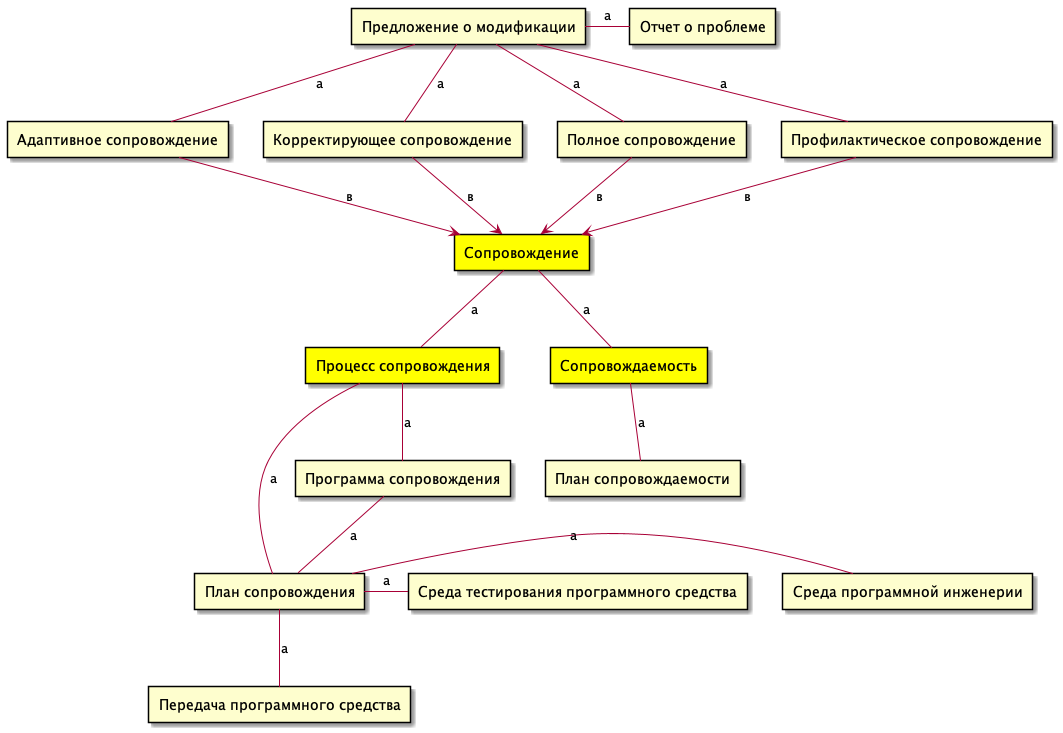
\includegraphics{images/thesaurus}
        }
    \end {center}\label{fig:thesaurus_img}
\end {figure}

    %! Author = vladislav.yaroshchuk
%! Date = 10/10/2021

\pagebreak


\section{Определение номенклатуры документов.}

Шаблоном процессов сопровождения и их документирования был выбран проект QEMU\cite{qemu,qemucontribute}.
Ниже представлена упрощенная диаграмма процесса сопровождения.

\begin{figure}[ht]
    \begin{center}
        \scalebox{0.4}{
            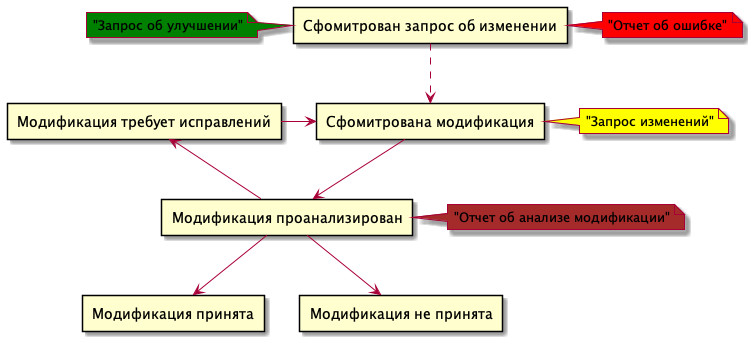
\includegraphics{images/maintenance_process}
        }
    \end {center}\label{fig:maintenance_process}
\end {figure}

Таким образом, получаем список документов:

\begin{itemize}
    \item План сопровождения -- описывает методы сопровождения, необходимые ресурсы и работы применительно к сопровождению.

    \item Отчет о проблеме -- описывает обнаруженную в продукте проблему

    \item Запрос об улучшении -- описывает требования к улучшению продукта, но не конкретные изменения

    \item Описание модификации -- описывает изменения в продукте, предполагаемые к включению в следующей версии продукта

    \item Отчет об анализе модификации -- описывает мнение отвественного (авторитетного) лица касательно Модификации

    \item Отчет об изменениях в версии -- описывает изменения в продукте в сравнении с предыдущей версией
\end{itemize}

    %! Author = vladislav.yaroshchuk
%! Date = 10/10/2021

\pagebreak
\section{Формирование требований к содержанию и оформлению, разработка шаблонов документов и примеров их заполнения}
    %! Author = vladislav.yaroshchuk
%! Date = 10/10/2021

\pagebreak


\section{Разработка регламента работы с документами.}

\subsection{Участники процесса сопровождения}

\begin{itemize}
    \item Старший сопровождающий (СТС) -- отвественное за продукт лицо
    \item Сопровождающий (С) -- представитель продукта, отвественное за продукт или часть продукта лицо
    \item Пользователь (П) -- лицо, использующее продукт
    \item Разработчик (РЗ) -- лицо, вносящее изменения в продукт
\end{itemize}

Примечание: так как за основу взят процесс сопровождения с исходным кодом, одно лицо может совмещать все четыре роли, приведенные выше.

\subsection{Регламент работы с документами}

\begin{center}
    \begin{longtable}{|p{3cm}|p{3.3cm}|p{3cm}|p{3cm}|p{3cm}|}
        \caption{Регламент работы с документами} \\
        \hline
        Документ                     & Инициирование & Создание      & Согласование \par и утверждение & Использование \\
        \hline
        План сопровождения           & СТС           & С, СТС        & СТС                             & П, РЗ, С, СТС \\
        \hline
        Отчет о проблеме             & П, РЗ, С, СТС & П, РЗ, С, СТС & С, СТС                          & П, РЗ, С, СТС \\
        \hline
        Запрос об улучшении          & П, РЗ, С, СТС & П, РЗ, С, СТС & С, СТС                          & П, РЗ, С, СТС \\
        \hline
        Описание модификации         & РЗ, С, СТС    & РЗ, С, СТС    & С, СТС                          & П, РЗ, С, СТС \\
        \hline
        Отчет об анализе модификации & С, СТС        & С, СТС        & С, СТС                          & П, РЗ, С, СТС \\
        \hline
        Отчет об изменениях в версии & С, СТС        & С, СТС        & СТС                             & П, РЗ, С, СТС \\
        \hline
    \end{longtable}
\end{center}

% Заключение
    %! Author = vladislav.yaroshchuk
%! Date = 10/10/2021

\pagebreak
\specialsection{Заключение}

В результате выполнения практической работы были изучены стандарты документирования и библиотеками лучших практик по созданию, поддержанию программного обеспечения на этапе \enquote{Программирование программных средств} его жизненного цикла.
Сформирован перечень требований и стандартов, необходимых для документирования данного этапа жизненного цикла, номенклатура документов и регламент работы с документами для этапа
\enquote{Сопровождение и техническая поддержка} жизненного цикла программного обеспечения.

% Ссыки на источники
    %! Author = vladislav.yaroshchuk
%! Date = 10/10/2021

% Библиография в cpsconf стиле
% Аргумент {1} ниже включает переопределенный стиль с выравниванием слева
\begin{thebibliography}{1}
    \bibitem{voc} Griffin D.W., Lim J.S. \flqq Multiband excitation vocoder\frqq. IEEE ASSP-36 (8), 1988, pp. 1223-1235.
    \bibitem{vo2} Griffin D.W., Lim J.S. \flqq Multiband excitation vocoder\frqq. IEEE ASSP-36 (8), 1988, pp. 1223-1235.
\end{thebibliography}

\end{document}